Se simularon las funciones descritas en la Tabla (\ref{fn}).
\begin{table}[H]
\centering
\begin{tabular}{@{}c@{}}
\toprule
Función \\ \midrule
$A\cdot Cos(2\pi \cdot 1.5kHz \cdot t)$ \\
Triangular simétrica 1.5kHz de pico $V_{MAX}$ \\
3/2 Seno amplitud VMAX 1.5kHz \\ \bottomrule
\end{tabular}
\caption{Funciones simuladas.}
\label{fn}
\end{table}

Se determinó que el valor máximo de amplitud de entrada al sistema es de $5 \ V$, el cual es el mínimo entre los dos valores limitantes: máxima entrada al CD4066 y límite mínimo de distorsión. Además, los límites de tensión de alimentación recomendados son $18 \ V$ de la hoja de datos del Sample and Hold.

Para hallar los valores óptimos de $A$, $F_s$ y $DT$ se simuló utilizando \textbf{LTSpiceXVII} las curvas de entrada y salida del sistema variando simultáneamente los valores de las tres variables, previamente fijando los rangos entre las mismas cambian. Estos rangos son de $1 \ V$ a $5 \ V$ para $A$, $21 \ kHz$ (para cumplir con el doble de la frecuencia de corte del filtro recuperador) a $25 \ kHz$ (límite del oscilador) y de $5\%$ (límite del oscilador) a $50\%$ (limite por consigna) para el duty cycle. Finalmente, se utilizó el siguiente script en \textbf{Python} para hallar el valor de los tres parámetros tal que la distorsión a la salida respecto a la entrada sea la mínima, computando la correlación entre las dos señales.
\begin{figure}[H]
\centering
\scalebox{0.75}{\lstinputlisting{../Ejercicio-6/Python/spiceanal.py}}
\end{figure}

Se obtuvieron los siguientes resultados:
\begin{figure}[H]
\centering
	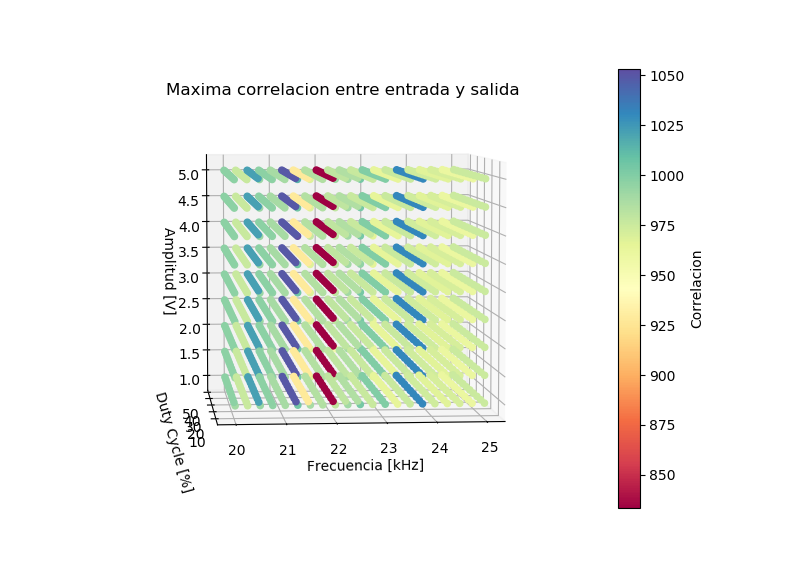
\includegraphics[width=0.8\linewidth]{ImagenesEjercicio6/scatter_sh_seno.png}
	\caption{Scatterplot de las simulación para \textbf{senoidal con S\&H}.}
	\label{seno_sh}
\end{figure}

\begin{figure}[H]
\centering
	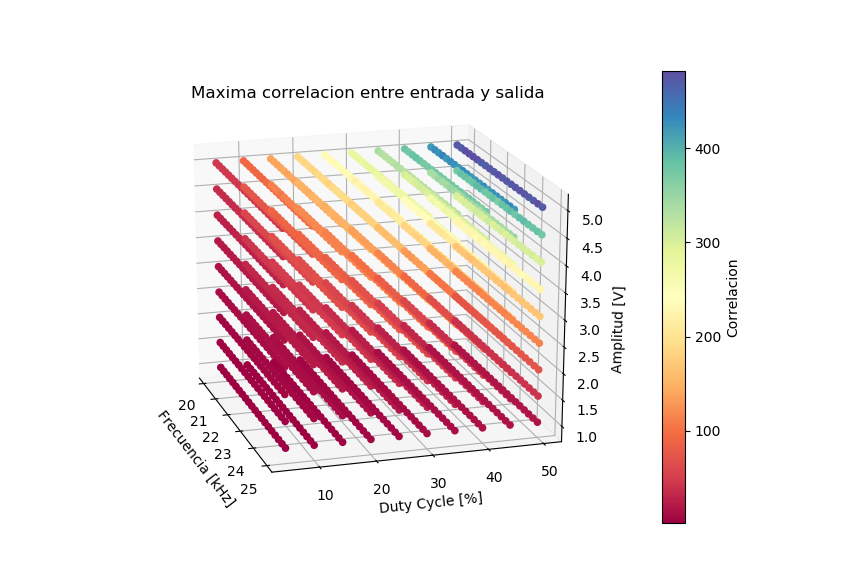
\includegraphics[width=0.8\linewidth]{ImagenesEjercicio6/scatter_llave_seno.png}
	\caption{Scatterplot de las simulación para la \textbf{senoidal con llave analógica}.}
	\label{seno_llave}
\end{figure}

\begin{figure}[H]
\centering
	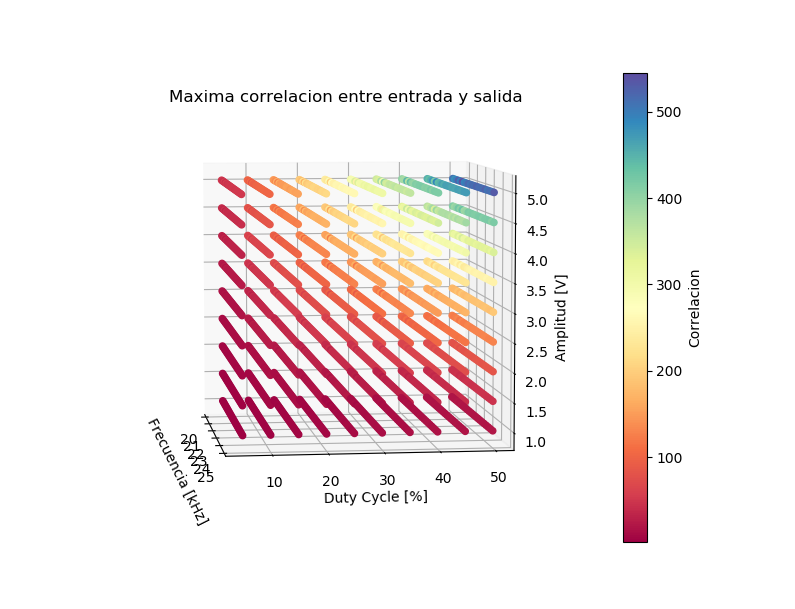
\includegraphics[width=0.8\linewidth]{ImagenesEjercicio6/scatter_llave_triang.png}
	\caption{Scatterplot de las simulación para la \textbf{triangular con llave analógica}.}
	\label{triang_llave}
\end{figure}

\begin{figure}[H]
\centering
	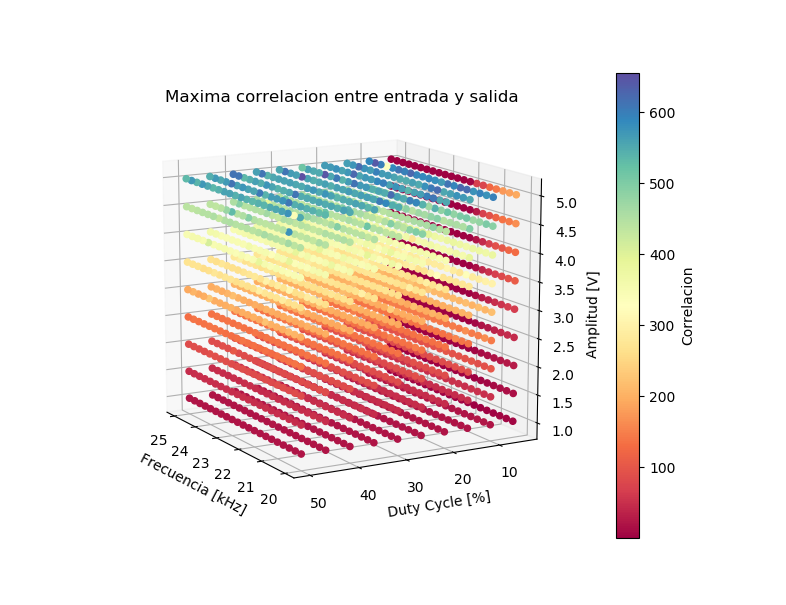
\includegraphics[width=0.8\linewidth]{ImagenesEjercicio6/scatter_sh_triang.png}
	\caption{Scatterplot de las simulación para la \textbf{triangular con S\&H}.}
	\label{triang_sh}
\end{figure}

\begin{figure}[H]
\centering
	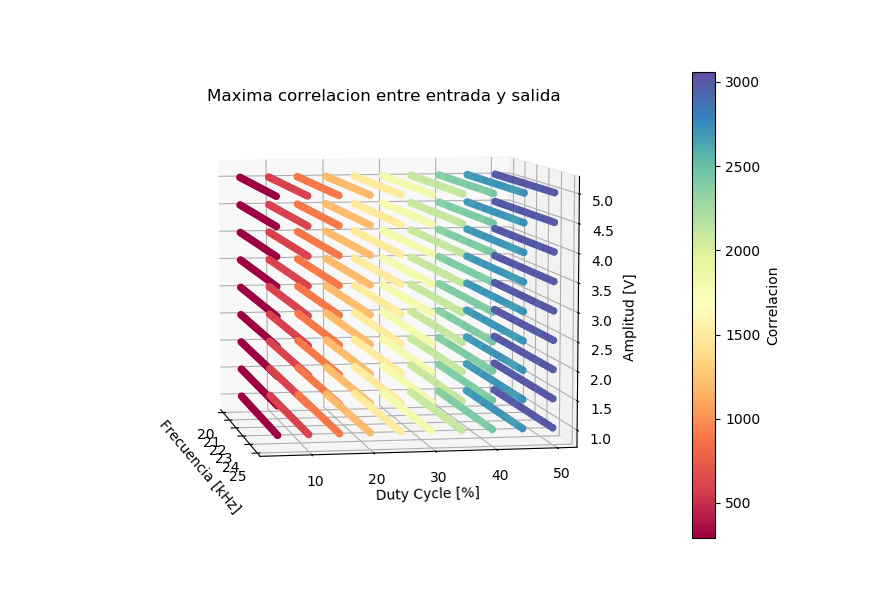
\includegraphics[width=0.8\linewidth]{ImagenesEjercicio6/scatter_llave_sen32.png}
	\caption{Scatterplot de las simulación para el \textbf{seno 3/2 con llave analógica}.}
	\label{sen32_llave}
\end{figure}

\begin{figure}[H]
\centering
	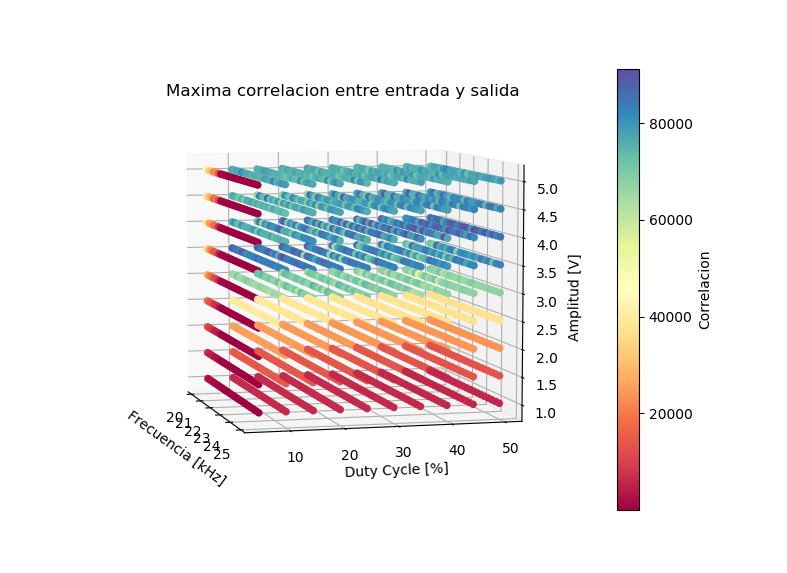
\includegraphics[width=0.8\linewidth]{ImagenesEjercicio6/scatter_sh_sen32.png}
	\caption{Scatterplot de las simulación para el \textbf{seno 3/2 con S\&H}.}
	\label{sen32_sh}
\end{figure}

De esta forma se efectuaron las siguientes tablas con los parámetros para la menor distorsión para cada circuito junto a la relación entre la potencia a la salida versus la salida a la entrada, es decir, $P_r = \frac{P_{out}}{P_{in}}$:
\begin{multicols}{2}
\begin{table}[H]
\centering
\begin{tabular}{ccccc}
\hline
$\mathbf{Entrada}$  & $\mathbf{A \ [V]}$ & $\mathbf{F_s \ [Hz]}$ & $\mathbf{DT \ [\%]}$ & $P_r$\\ \hline
\textbf{Coseno}     & 5                 & 24000                 & 20         &      1.0196     \\
\textbf{3/2 Seno}   & 4                & 23250                 & 40           &    0.7991     \\
\textbf{Triangular} & 5                  & 25000                 & 45          &       0.6585 	\\ \hline
\end{tabular}
\caption{Circuito con Sample and Hold.}
\label{tab:res1}
\end{table}
\begin{table}[H]
\centering
\begin{tabular}{ccccc}
\hline
$\mathbf{Entrada}$  & $\mathbf{A \ [V]}$ & $\mathbf{F_s \ [Hz]}$ & $\mathbf{DT \ [\%]}$ &$P_r$ \\ \hline
\textbf{Coseno}     & 5                  & 25000                 & 50       &     0.2305       \\
\textbf{3/2 Seno}   & 4                  & 22250                 & 45        &      0.5781     \\
\textbf{Triangular} & 5                  & 21250                 & 50         &    0.1489      \\ \hline
\end{tabular}
\caption{Circuito con llave analógica.}
\label{tab:res2}
\end{table}
\end{multicols}


\subsubsection{Simulaciones con Python}
Se utilizó el framework de \textbf{GNURadio} para programar cada módulo del sistema encerrado en una interfaz gráfica, la cual brinda la posibilidad de visualizar tanto la señal en tiempo como su espectro en cada nodo del sistema en el mismo momento. Se puede elegir entre señales sinusoidales, triangulares, 3/2 seno o moduladas AM como entrada, señales cuyo estudio es de interés.

Se realizaron las simulaciones de las funciones en la Tabla (\ref{fn}) con los parámetros que obtenidos y detallados en las Tablas (\ref{tab:res1}) y (\ref{tab:res2}).

\begin{figure}[H]
	\begin{subfigure}{.5\textwidth}
	\centering
	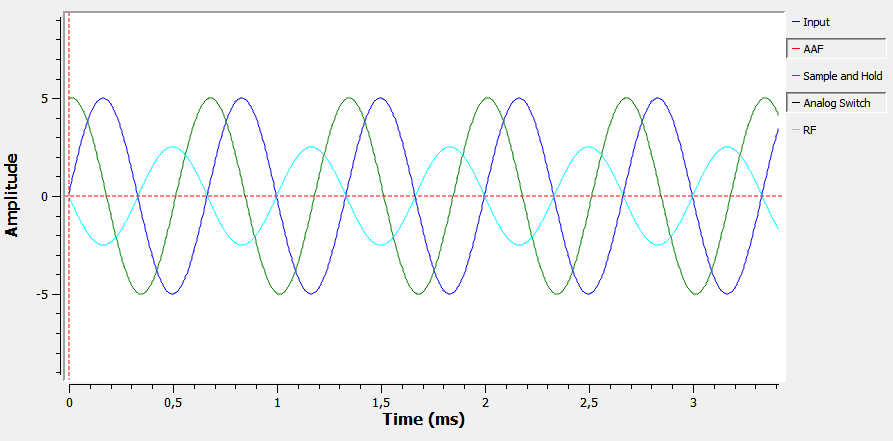
\includegraphics[width=\textwidth]{SimulacionesGNURADIO/Condiciones_optimas/COSENO_TIEMPO_LLAVE_BC.PNG}
	\end{subfigure}	
	\begin{subfigure}{.5\textwidth}
	\centering
	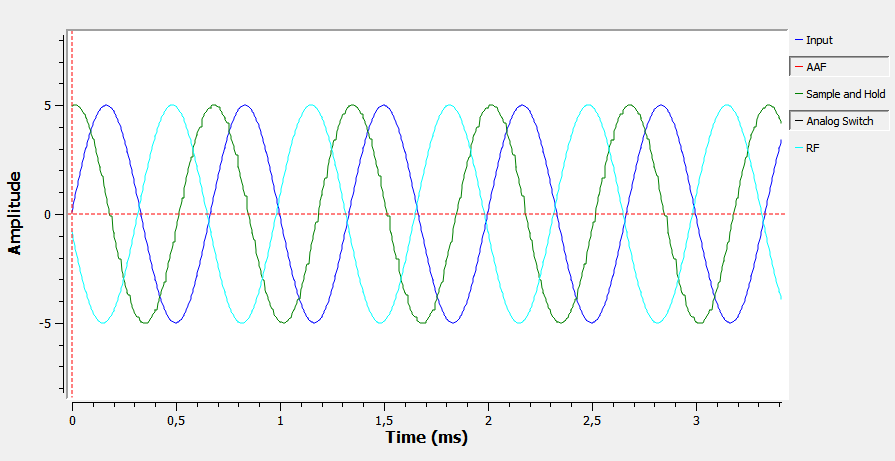
\includegraphics[width=\textwidth]{SimulacionesGNURADIO/Condiciones_optimas/COSENO_TIEMPO_SAMPLE_AND_HOLD_BC.PNG}
	\end{subfigure}
	
	\begin{subfigure}{.5\textwidth}
	\centering
	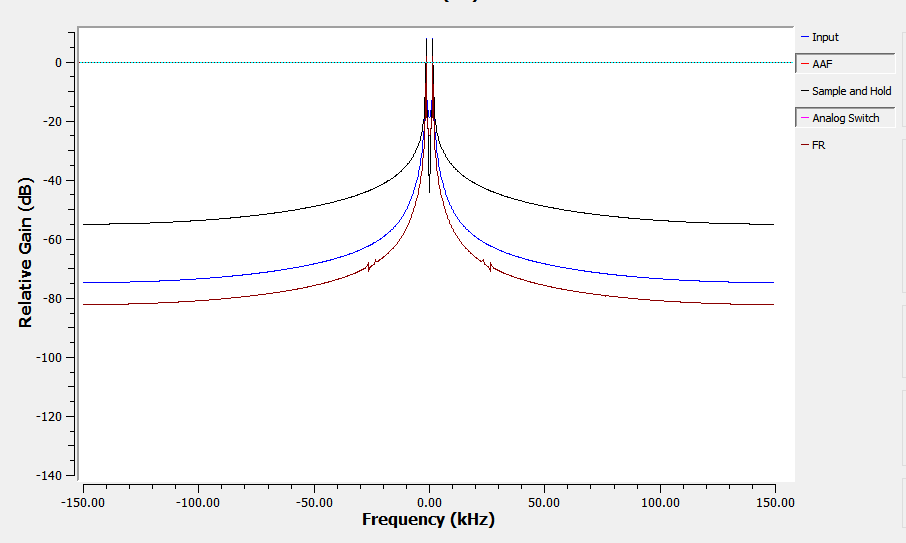
\includegraphics[width=\textwidth]{SimulacionesGNURADIO/Condiciones_optimas/COSENO_FFT_LLAVE_BC.PNG}
	\caption{Sistema con llave analógica.}
	\end{subfigure}
	\begin{subfigure}{.5\textwidth}
	\centering
	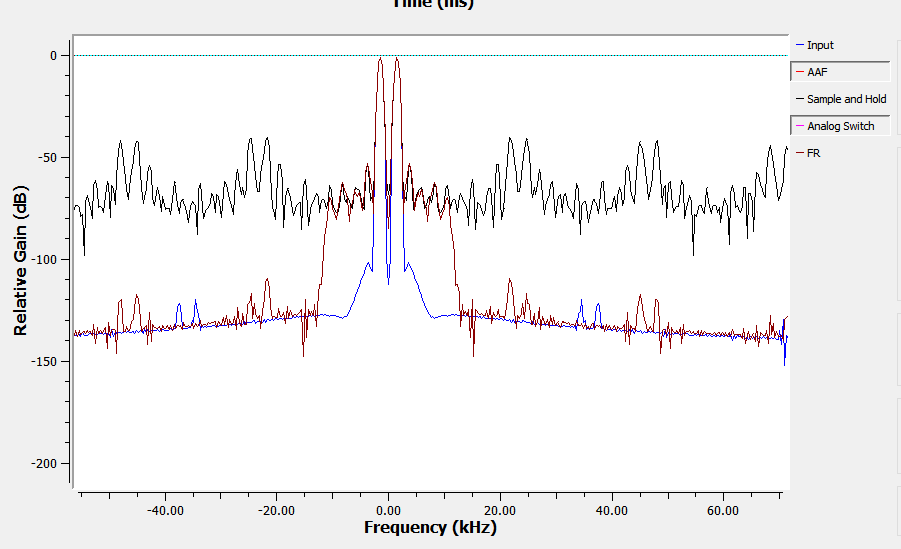
\includegraphics[width=\textwidth]{SimulacionesGNURADIO/Condiciones_optimas/COSENO_FFT_SAMPLE_AND_HOLD_BC.PNG}
	\caption{Sistema con sample and hold.}	
	\end{subfigure}
	\caption{Señal cosenoidal a través del sistema.}
\end{figure}


\begin{figure}[H]
	\begin{subfigure}{.5\textwidth}
	\centering
	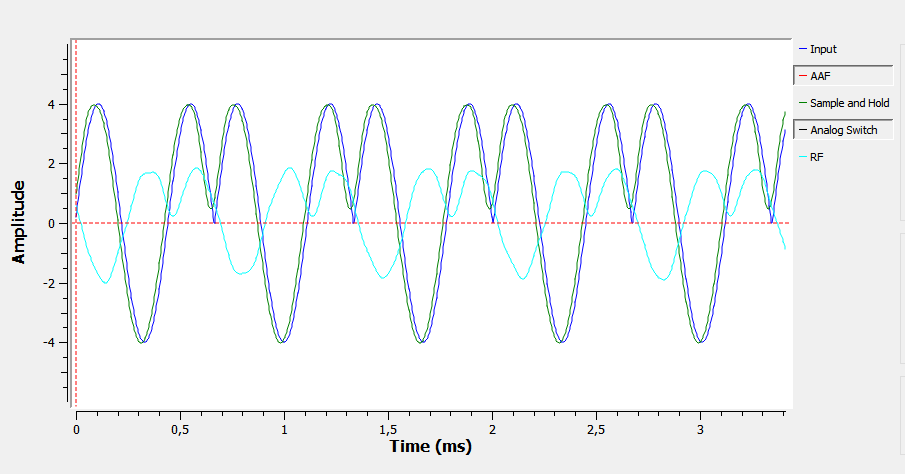
\includegraphics[width=\textwidth]{SimulacionesGNURADIO/Condiciones_optimas/SENO32_TIEMPO_LLAVE_BC.PNG}
	\end{subfigure}
	\begin{subfigure}{.5\textwidth}
	\centering

		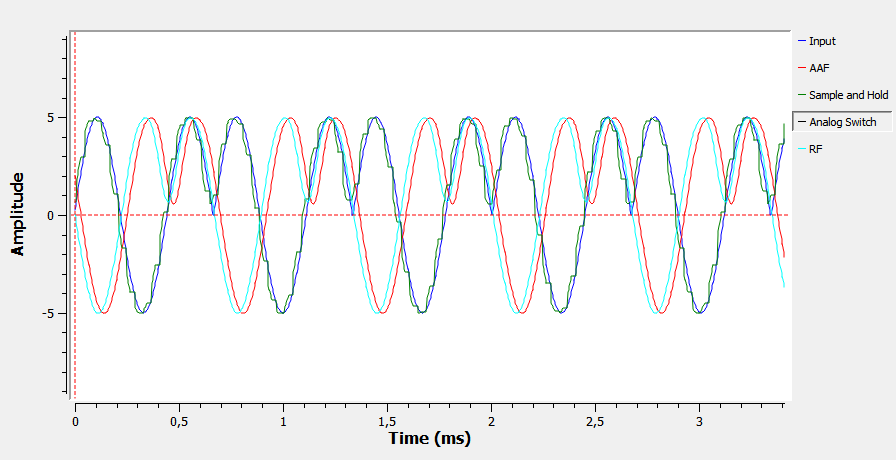
\includegraphics[width=\textwidth]{SimulacionesGNURADIO/Condiciones_optimas/SENO32_TIEMPO_SAMPLE_AND_HOLD_BC.PNG}
	\end{subfigure}
	
	\begin{subfigure}{.5\textwidth}
	\centering
	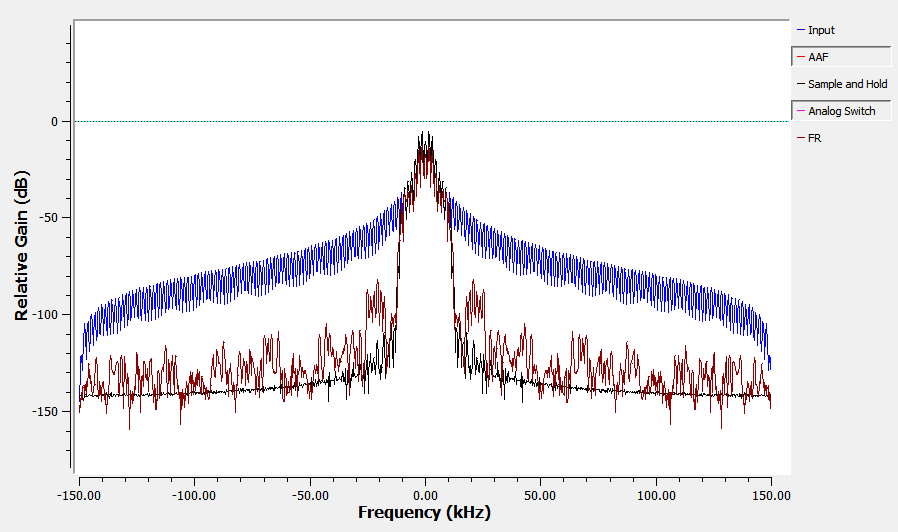
\includegraphics[width=\textwidth]{SimulacionesGNURADIO/Condiciones_optimas/SENO32_FFT_LLAVE_BC.PNG}
		\caption{Sistema con llave analógica.}	
	\end{subfigure}
	\begin{subfigure}{.5\textwidth}
	\centering
	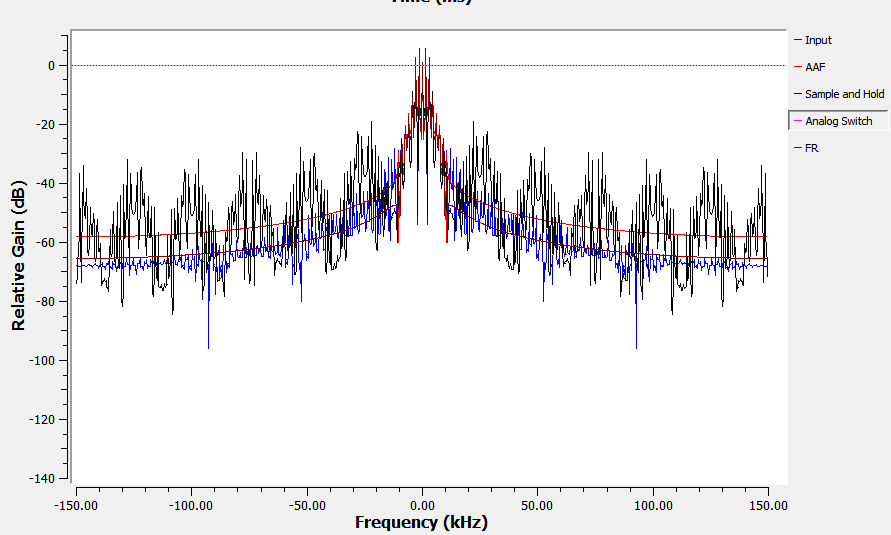
\includegraphics[width=\textwidth]{SimulacionesGNURADIO/Condiciones_optimas/SENO32_FFT_SAMPLE_AND_HOLD_BC.PNG}
		\caption{Sistema con sample and hold.}	
	\end{subfigure}
	\caption{Señal seno 3/2 a través del sistema.}
\end{figure}


\begin{figure}[H]
		\begin{subfigure}{.5\textwidth}
	\centering
	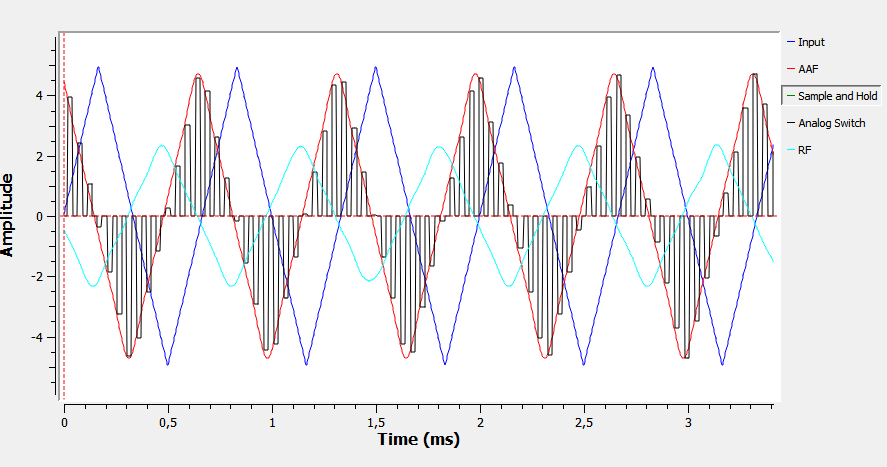
\includegraphics[width=\textwidth]{SimulacionesGNURADIO/Condiciones_optimas/TRIANGULAR_TIEMPO_LLAVE_BC.PNG}
	\end{subfigure}
	\begin{subfigure}{.5\textwidth}
	\centering

		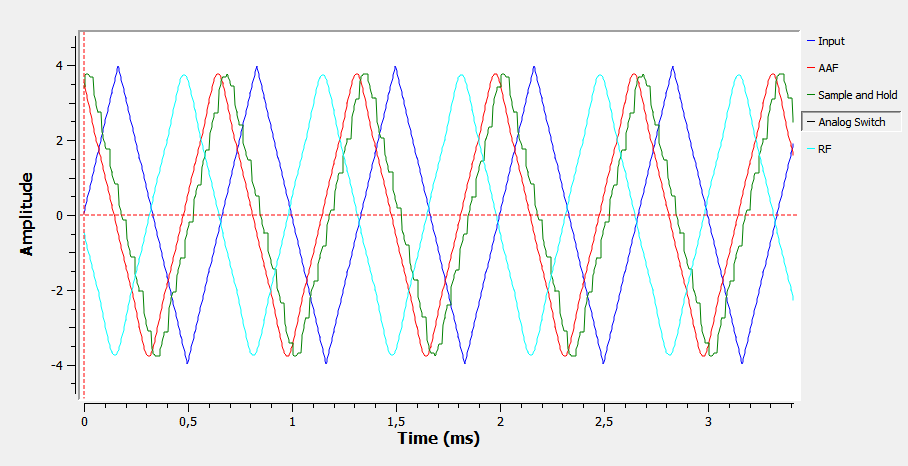
\includegraphics[width=\textwidth]{SimulacionesGNURADIO/Condiciones_optimas/TRIANGULAR_TIEMPO_SAMPLE_AND_HOLD_BC.PNG}
	\end{subfigure}
	
		\begin{subfigure}{.5\textwidth}
	\centering
	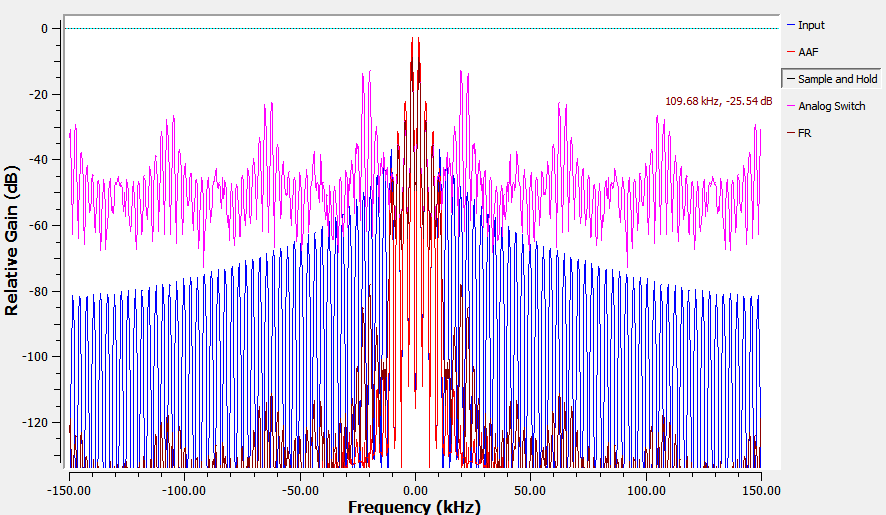
\includegraphics[width=\textwidth]{SimulacionesGNURADIO/Condiciones_optimas/TRIANGULAR_FFT_LLAVE_BC.PNG}
	\caption{Sistema con llave analógica.}		
	\end{subfigure}
	\begin{subfigure}{.5\textwidth}
	\centering
	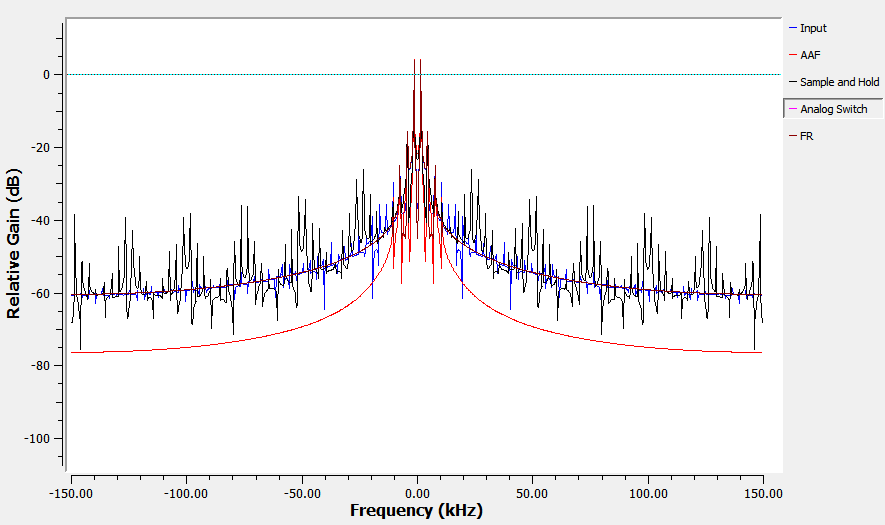
\includegraphics[width=\textwidth]{SimulacionesGNURADIO/Condiciones_optimas/TRIANGULAR_FFT_SAMPLE_AND_HOLD_BC.PNG}
	\caption{Sistema con sample and hold.}		
	\end{subfigure}
	
	\caption{Señal triangular a través del sistema.}
\end{figure}


\subsubsection{Simulaciones con LTSpice}
Para ambos sistemas se realizaron las simulaciones de las funciones en la Tabla (\ref{fn}) con los parámetros que obtenidos y detallados en las Tablas (\ref{tab:res1}) y (\ref{tab:res2}). A continuación se presenta una comparación temporal de la entrada y salida para cada uno de los casos analizados.

\begin{figure}[H]
	\begin{subfigure}{.5\textwidth}
	\centering
	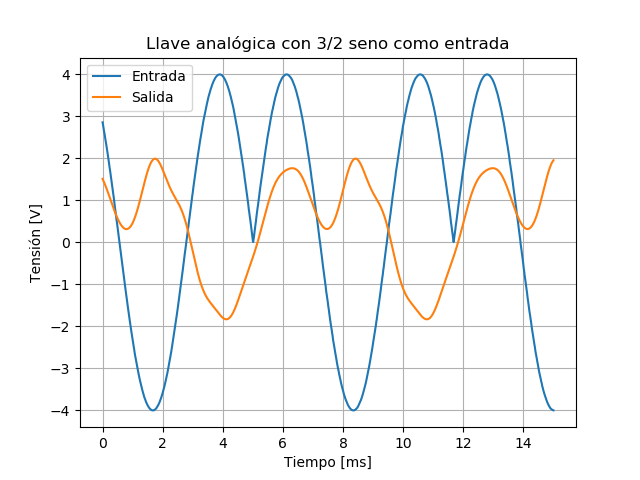
\includegraphics[width=\textwidth]{ImagenesEjercicio6/puntoa/LA - 3 2.png}
	\end{subfigure}	
	\begin{subfigure}{.5\textwidth}
	\centering
	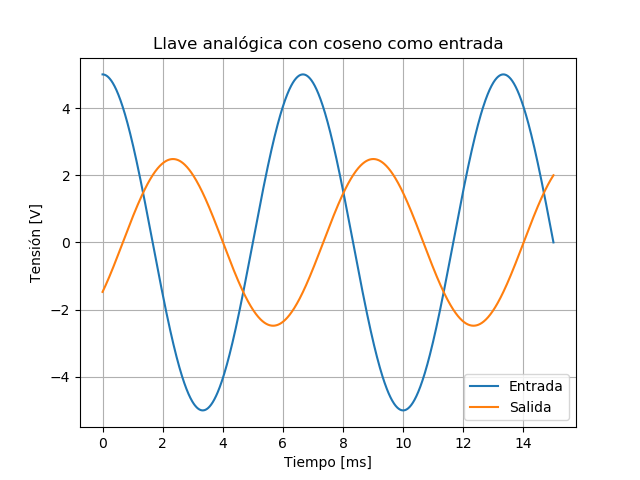
\includegraphics[width=\textwidth]{ImagenesEjercicio6/puntoa/LA - Cos.png}
	\end{subfigure}
	
	\begin{subfigure}{.5\textwidth}
	\centering
	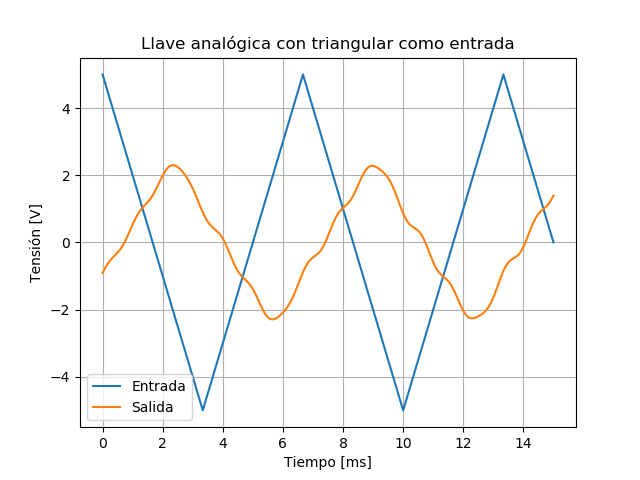
\includegraphics[width=\textwidth]{ImagenesEjercicio6/puntoa/LA - Tri.png}
	\end{subfigure}
	\begin{subfigure}{.5\textwidth}
	\centering
	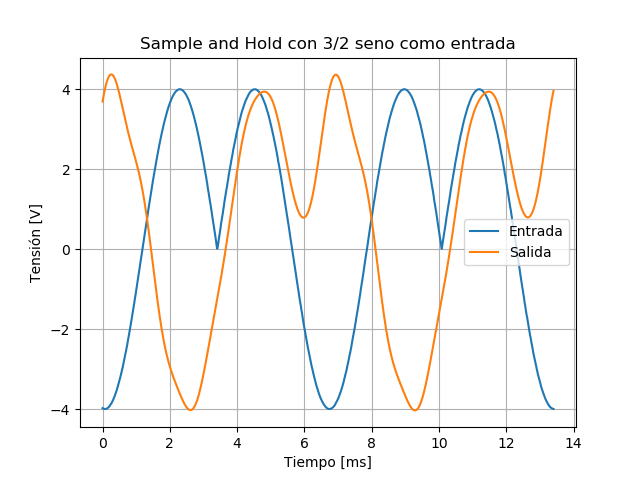
\includegraphics[width=\textwidth]{ImagenesEjercicio6/puntoa/SH - 3 2.png}
	\end{subfigure}
	
	\begin{subfigure}{.5\textwidth}
	\centering
	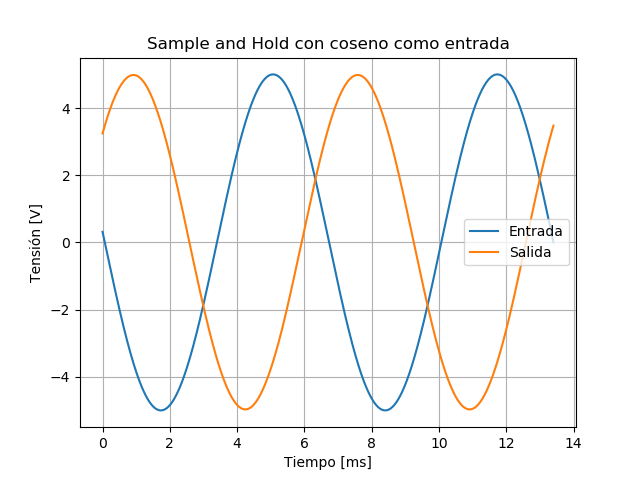
\includegraphics[width=\textwidth]{ImagenesEjercicio6/puntoa/SH - Cos.png}
	\end{subfigure}
	\begin{subfigure}{.5\textwidth}
	\centering
	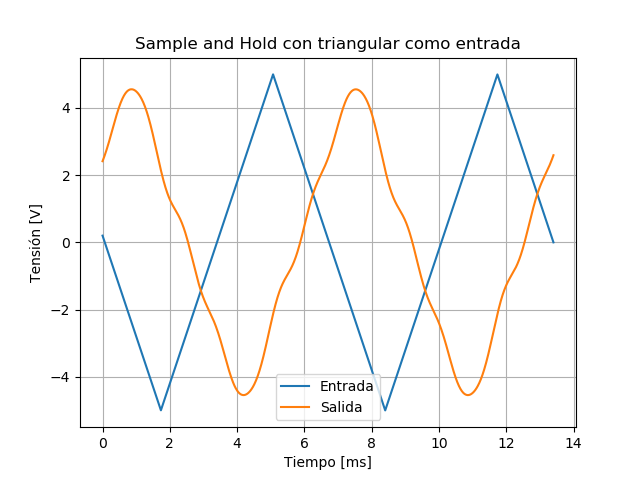
\includegraphics[width=\textwidth]{ImagenesEjercicio6/puntoa/SH - Tri.png}
	\end{subfigure}
\end{figure}

Es notable como la amplitud de las señales muestreadas solamente con sample and hold es casi igual a la amplitud de la señal original, dado que este tipo de muestreo es equivalente a un pseudo-muestreo instantáneo de duty cycle 100\%. En el caso de la señal muestreada solamente con la llave analógica, la amplitud a la salida es mucho menor que la amplitud a la entrada, al igual que la potencia a la salida versus la potencia a la entrada. Esto puede verse tanto en el tiempo como en la frecuencia. En el tiempo, al muestrear con una llave analógica se están introduciendo ceros a la señal original donde antes había valores distintos de cero, esto causa que la potencia de la señal se vea disminuida. En la frecuencia, se puede observar este efecto al tener en cuenta que el espectro de la señal se ve ponderada por el sinc.
Nuevamente, se realizaron las mismas simulaciones utilizando una frecuencia de entrada de $5 \ kHz$ y una frecuencia de sampleo de $15750 \ Hz$.

\begin{figure}[H]
	\begin{subfigure}{.5\textwidth}
	\centering
	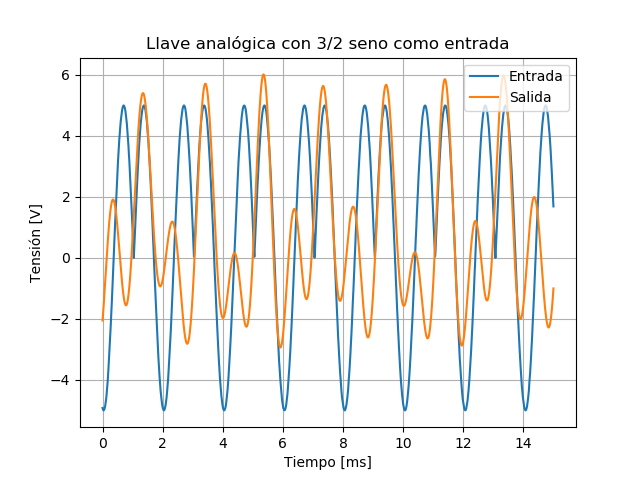
\includegraphics[width=\textwidth]{ImagenesEjercicio6/puntob1/LA - 3 2.png}
	\end{subfigure}	
	\begin{subfigure}{.5\textwidth}
	\centering
	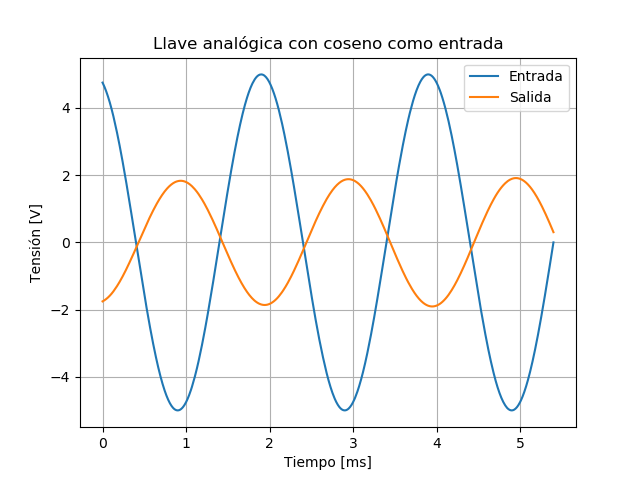
\includegraphics[width=\textwidth]{ImagenesEjercicio6/puntob1/LA - Cos.png}
	\end{subfigure}
	
	\begin{subfigure}{.5\textwidth}
	\centering
	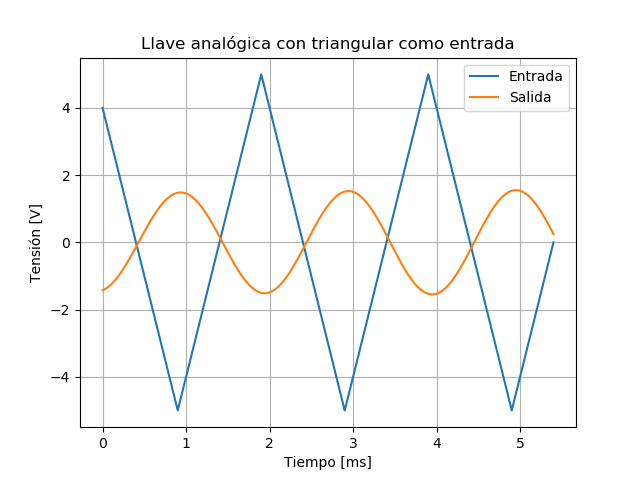
\includegraphics[width=\textwidth]{ImagenesEjercicio6/puntob1/LA - Tri.png}
	\end{subfigure}
	\begin{subfigure}{.5\textwidth}
	\centering
	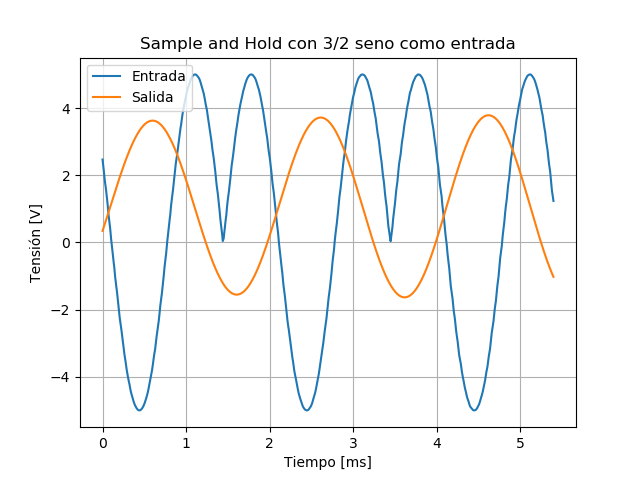
\includegraphics[width=\textwidth]{ImagenesEjercicio6/puntob1/SH - 3 2.png}
	\end{subfigure}
	
	\begin{subfigure}{.5\textwidth}
	\centering
	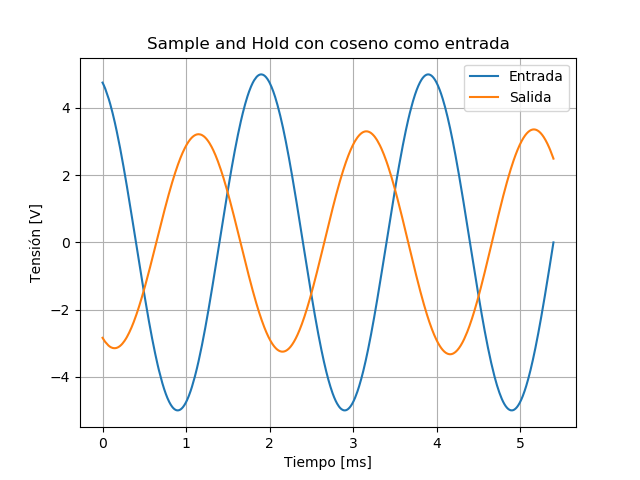
\includegraphics[width=\textwidth]{ImagenesEjercicio6/puntob1/SH - Cos.png}
	\end{subfigure}
	\begin{subfigure}{.5\textwidth}
	\centering
	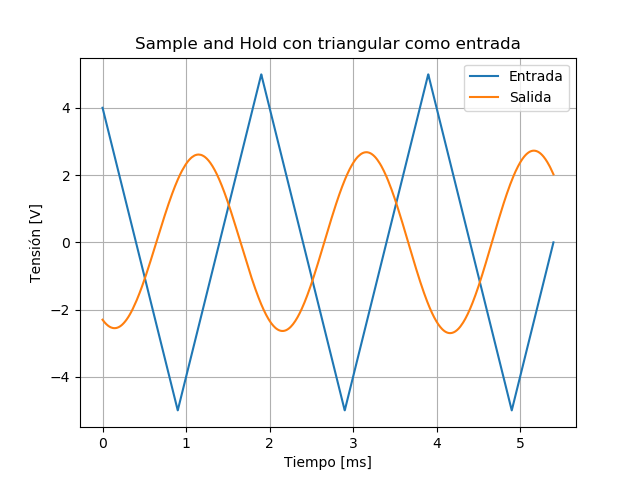
\includegraphics[width=\textwidth]{ImagenesEjercicio6/puntob1/SH - Tri.png}
	\end{subfigure}
\end{figure}

Para este caso, se observan aliases en la señal recuperada, dado que como la frecuencia de sampleo se encuentra por debajo de dos veces la frecuencia de corte del filtro anti-alias, al recuperar la señal no se logra segmentar correctamente el espectro de la señal original en banda base sino que se recupera también un sobrelapamiento de los espectros repetidos de la señal original.
Finalmente, con una frecuencia de entrada de $15750 \ Hz$ y una frecuencia de sampleo de $30 \ kHz$.

\begin{figure}[H]
	\begin{subfigure}{.5\textwidth}
	\centering
	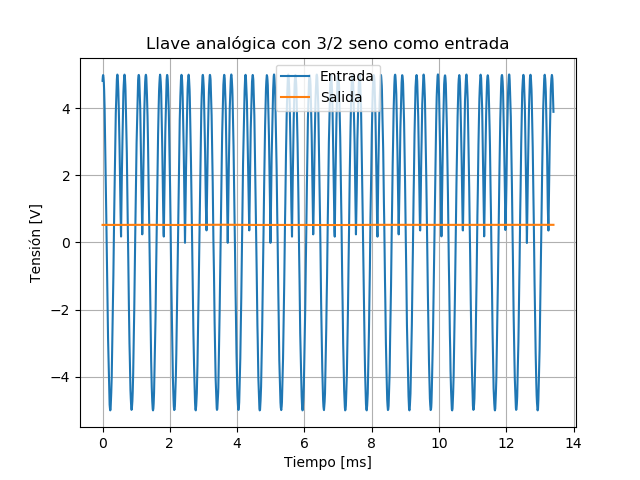
\includegraphics[width=\textwidth]{ImagenesEjercicio6/puntob2/LA - 3 2.png}
	\end{subfigure}	
	\begin{subfigure}{.5\textwidth}
	\centering
	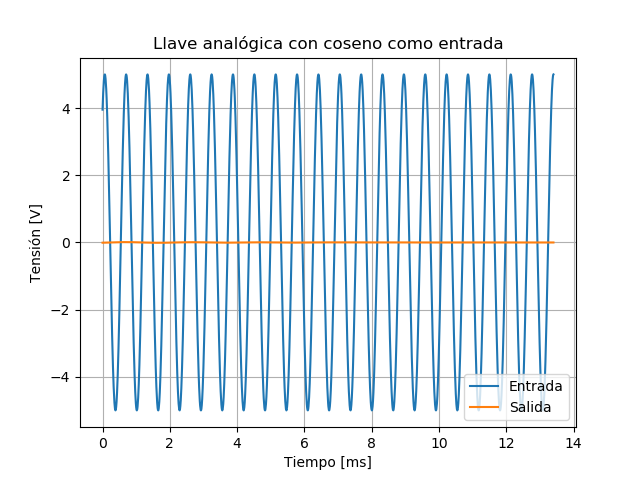
\includegraphics[width=\textwidth]{ImagenesEjercicio6/puntob2/LA - Cos.png}
	\end{subfigure}
	
	\begin{subfigure}{.5\textwidth}
	\centering
	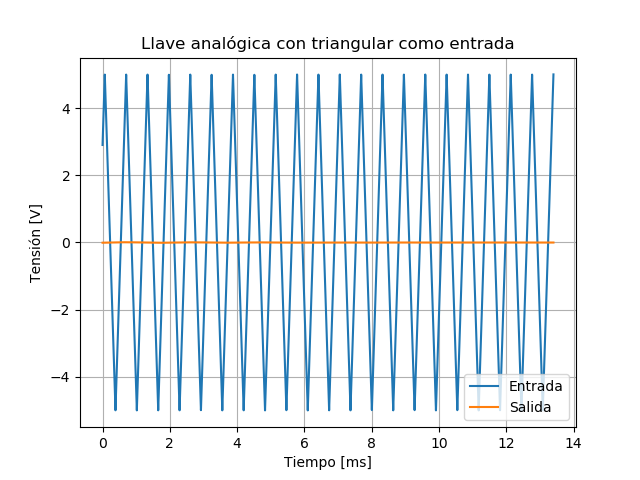
\includegraphics[width=\textwidth]{ImagenesEjercicio6/puntob2/LA - Tri.png}
	\end{subfigure}
	\begin{subfigure}{.5\textwidth}
	\centering
	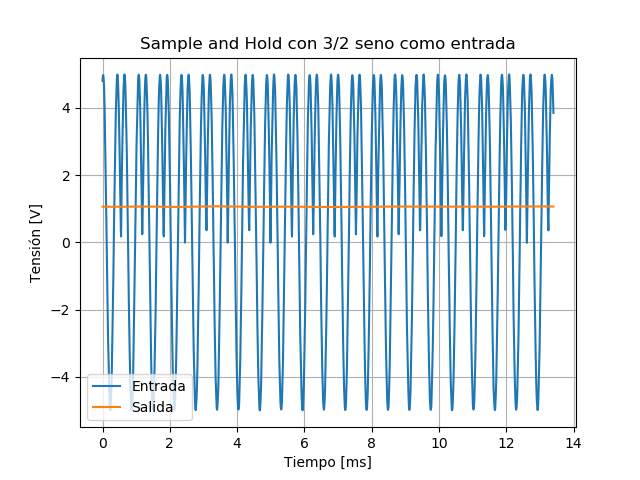
\includegraphics[width=\textwidth]{ImagenesEjercicio6/puntob2/SH - 3 2.png}
	\end{subfigure}
	
	\begin{subfigure}{.5\textwidth}
	\centering
	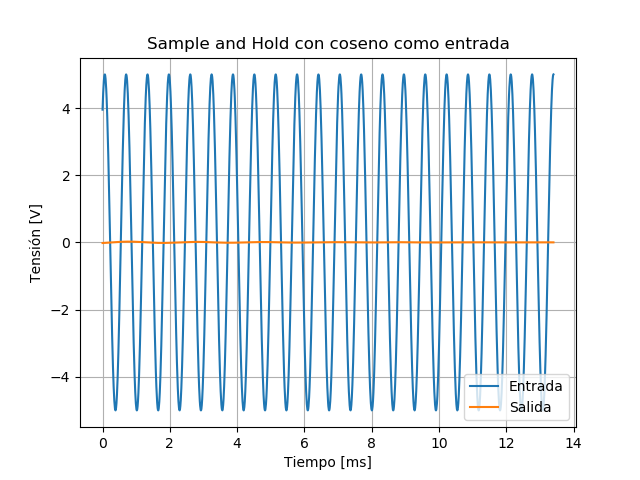
\includegraphics[width=\textwidth]{ImagenesEjercicio6/puntob2/SH - Cos.png}
	\end{subfigure}
	\begin{subfigure}{.5\textwidth}
	\centering
	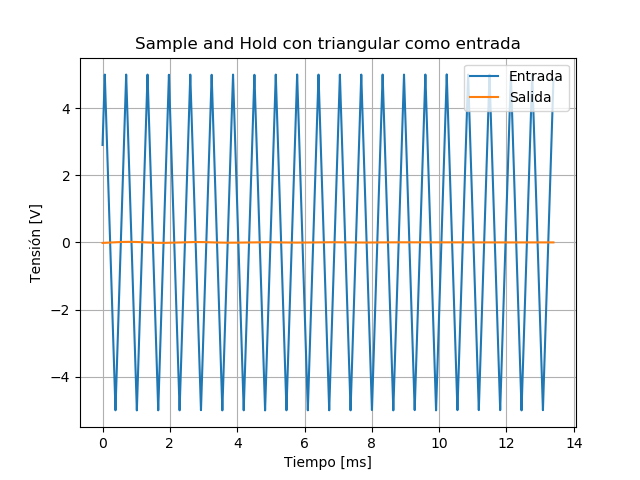
\includegraphics[width=\textwidth]{ImagenesEjercicio6/puntob2/SH - Tri.png}
	\end{subfigure}
\end{figure}

Se calcularon las potencias recuperadas en cada caso

\begin{table}[H]
\centering
\begin{tabular}{cccc}
\hline
\textbf{Sistema + Señal}  & \textbf{Potencia recuperada $f_{in}=5kHz$} & \textbf{Potencia recuperada $f_{in}=15.75kHz$} \\ \hline
\textbf{S\&H Coseno}     & 0.8282   & 2E-06\\
\textbf{S\&H Seno 3/2}   & 1.1599  & 0.1100\\
\textbf{S\&H Triangular} & 0.8989  & 3E-06\\
\textbf{Llave Coseno}     & 0.3889 & 6E-06 \\
\textbf{Llave Seno 3/2}   & 0.5470  & 0.0203\\
\textbf{Llave Triangular} & 0.2701	& 5E-06\\ \hline
\end{tabular}
\caption{Circuito con Sample and Hold.}
\label{tab:res3}
\end{table}

Se puede observar que la potencia recuperada para los últimos casos es casi nula, dado que el filtro anti-alias posee una gran atenuación para frecuencias mayores o iguales a $f_a$, por lo que la señal de entrada a la salida del filtro es ínfima.

Se simuló el caso en el que la señal cosenoidal posee misma frecuencia que la de sampleo, ambas por debajo de la frecuencia de corte del filtro anti-alias, generando las salidas que se observan a continuación.

\begin{figure}[H]
	\begin{subfigure}{.5\textwidth}
	\centering
	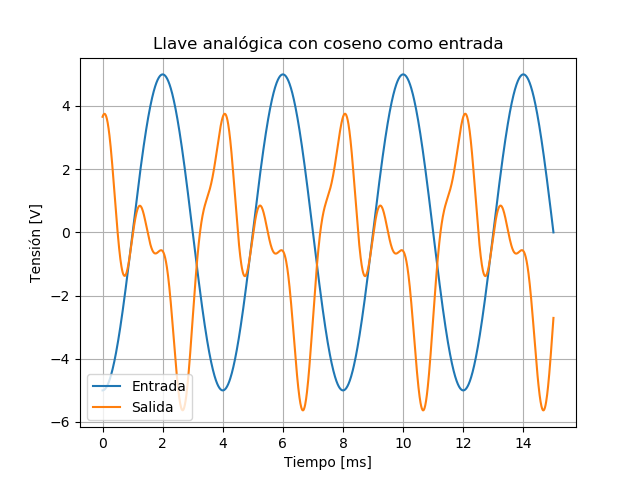
\includegraphics[width=\textwidth]{ImagenesEjercicio6/puntoc-d/LA - Cos.png}
	\end{subfigure}
	\begin{subfigure}{.5\textwidth}
	\centering
	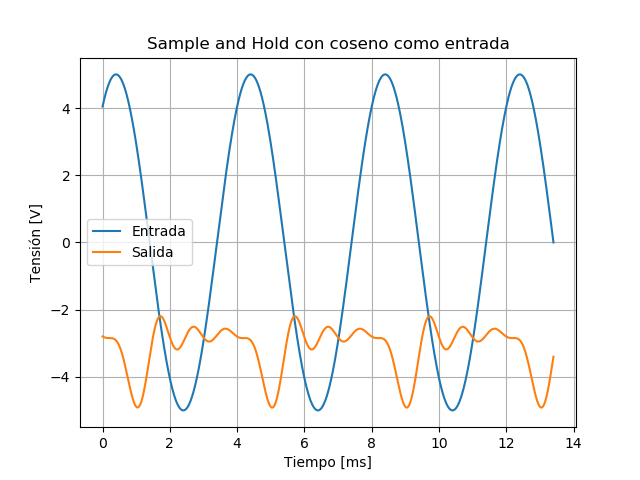
\includegraphics[width=\textwidth]{ImagenesEjercicio6/puntoc-d/SH - Cos.png}
	\end{subfigure}
\end{figure}

Estas distorsiones se deben a que $f_S < f_N$. Además, dado que el $f_P$ del filtro recuperador es mayor a la de muestreo, no solamente hay superposición de espectros sino que también hay alias.

%\begin{equation*}
%	\mathcal{F}_{N} \left( \omega \right) = \frac{A \tau}{T} \sum_{n=-\infty}^{\infty} sinc \left( \frac{n \tau \omega_S}{2 \pi} \right) \mathcal{F} \left( \omega - n \omega_S \right)
%\end{equation*}
%
%\begin{equation*}
%	\mathcal{F}_{N} \left( \omega_S \right) = \frac{A \tau}{T} \sum_{n=-\infty}^{\infty} sinc \left( \frac{n \tau \omega_S}{2 \pi} \right) \mathcal{F} \left( \left( 1 - n \right) \omega_S \right)
%\end{equation*}
%
%\begin{equation*}
%	\mathcal{F}_{N} \left( \omega_S \right) = \frac{A \tau}{T} \sum_{k=-\infty}^{\infty} sinc \left( \frac{ \left( 1 - k \right) \tau \omega_S}{2 \pi} \right) \mathcal{F} \left( k \omega_S \right)
%\end{equation*}

Finalmente se tomaron nuevamente ambos sistemas para la entrada triangular y para la 3/2 seno y se fue variando la frecuencia de sampleo. De esta forma, llegando a que esta última variable sea de $11 \ kHz$, se obtuvieron los siguientes resultados:
\begin{figure}[H]
\centering
	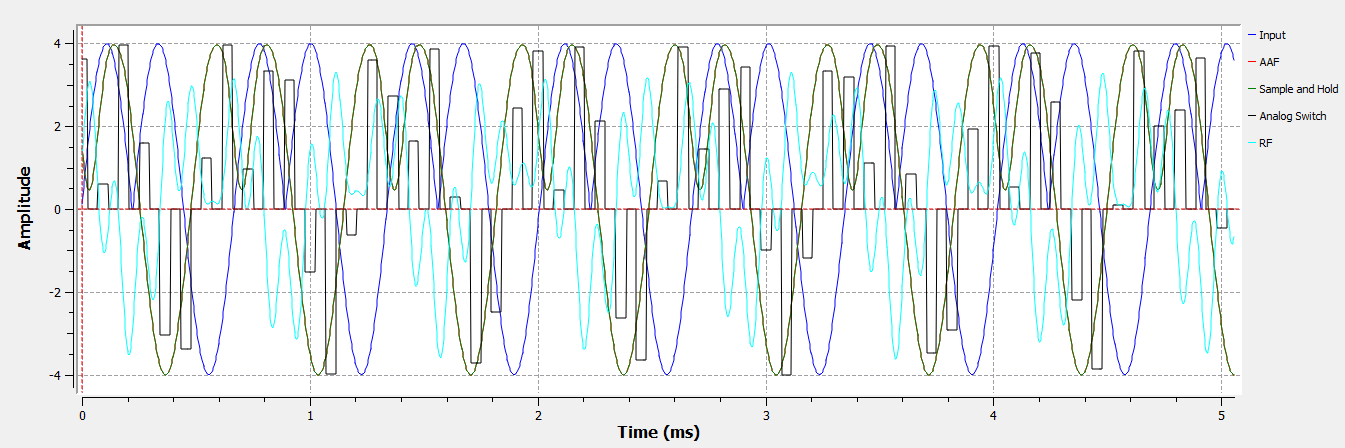
\includegraphics[width=0.8\linewidth]{ImagenesEjercicio6/6d-32LA11k.png}
	\caption{Llave analógica con 3/2 seno.}
	\label{fig:32la}
\end{figure}
\begin{figure}[H]
\centering
	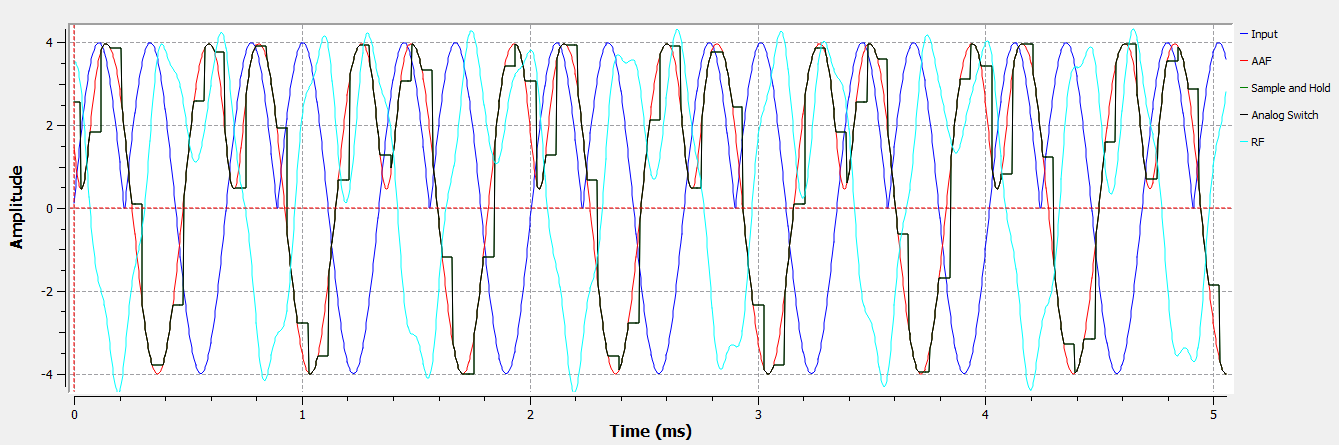
\includegraphics[width=0.8\linewidth]{ImagenesEjercicio6/6d-32SH11k.png}
	\caption{Sample and Hold con 3/2 seno.}
	\label{fig:32sh}
\end{figure}
\begin{figure}[H]
\centering
	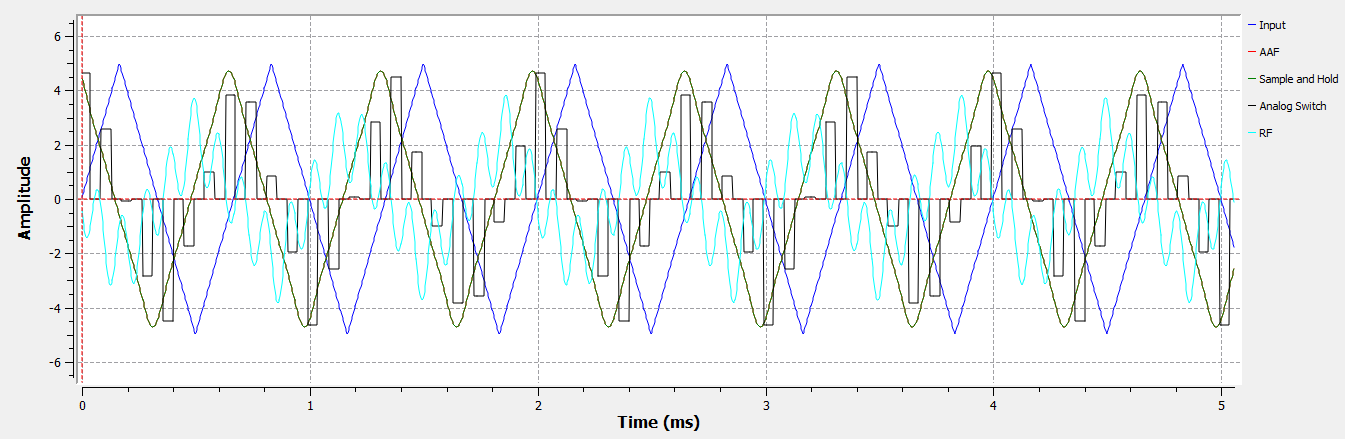
\includegraphics[width=0.8\linewidth]{ImagenesEjercicio6/6d-TRLA11k.png}
	\caption{Llave analógica con triangular.}
	\label{fig:trla}
\end{figure}
\begin{figure}[H]
\centering
	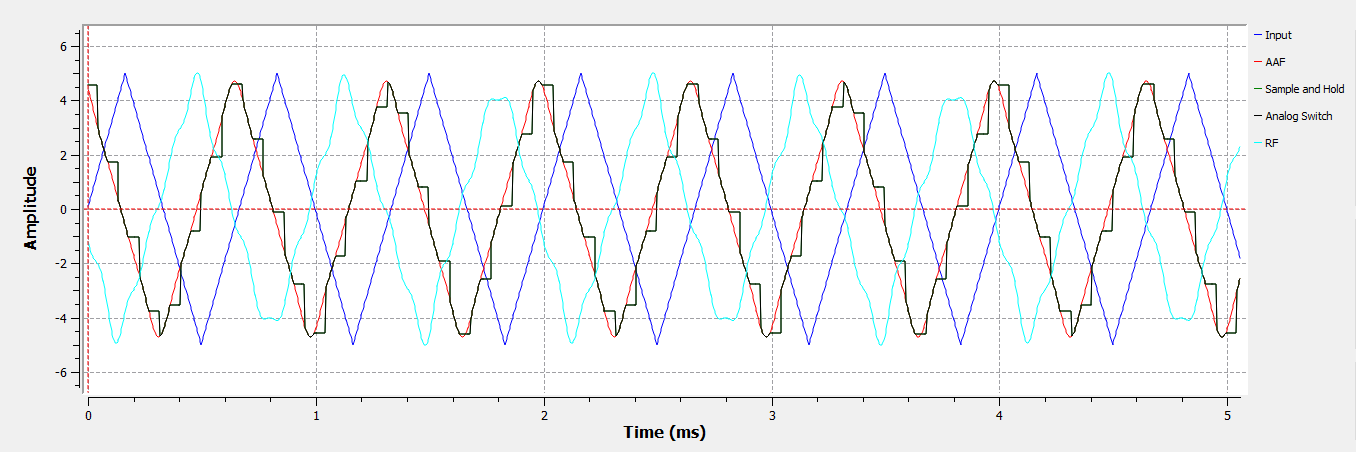
\includegraphics[width=0.8\linewidth]{ImagenesEjercicio6/6d-TRSH11k.png}
	\caption{Sample and Hold con triangular.}
	\label{fig:trsh}
\end{figure}

Dado que la frecuencia de muestreo debe ser superior al doble de la de Nyquist, y dicha condición no está siendo cumplida, se puede observar como la señal recuperada a la salida del sistema se encuentra distorsionada. Esto se debe a la superposición de espectros repetidos en frecuencia de la señal muestrada. Si se trabaja con una mayor al doble de la frecuencia de Nyquist, se garantiza que estos espectros no se superponen. Cabe destacar que al comparar los resultados de ambos sistemas, es notable que el Sample and Hold presenta mejores resultados que la llave analógica dado que el primer sistema mantiene constante la señal en ciertos instantes mientras que el segundo simplemente toma valores nulos, generando una mayor perdida de información.
\subsection{PCB}
Se realizó el diseño de la placa en Altium, teniendo en cuenta los criterios de diseño vistos en la clase, utilizando esquematicos multisheet y pcb dobel faz.
\begin{figure}[H]
\centering
	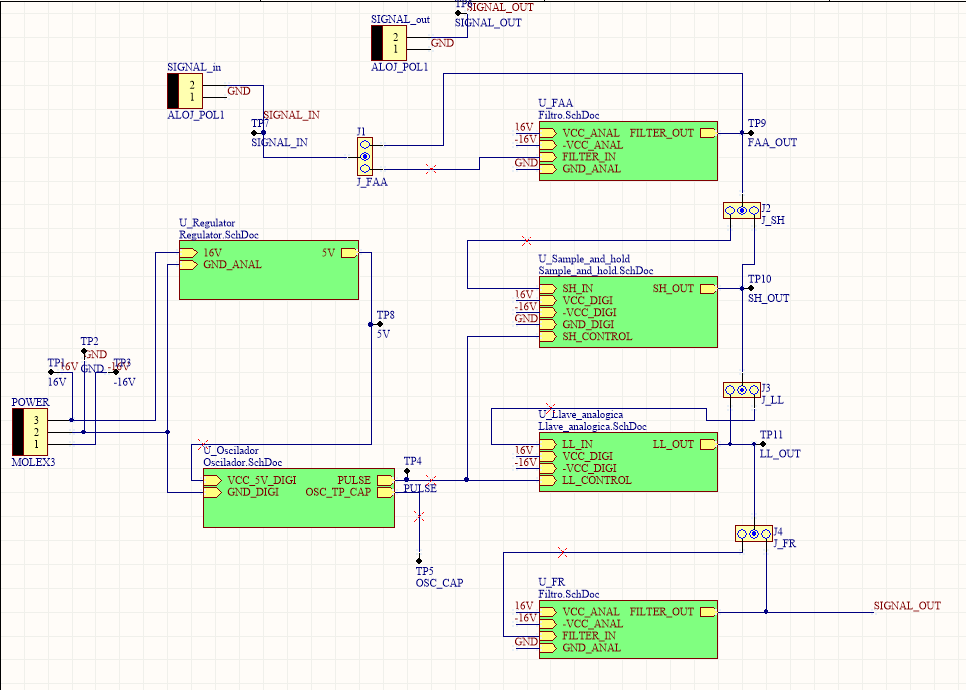
\includegraphics[width=0.8\linewidth]{ImagenesEjercicio6/main.png}
	\caption{Esquemático altium.}
	\label{fig:esq}
\end{figure}
\begin{figure}[H]
\centering
	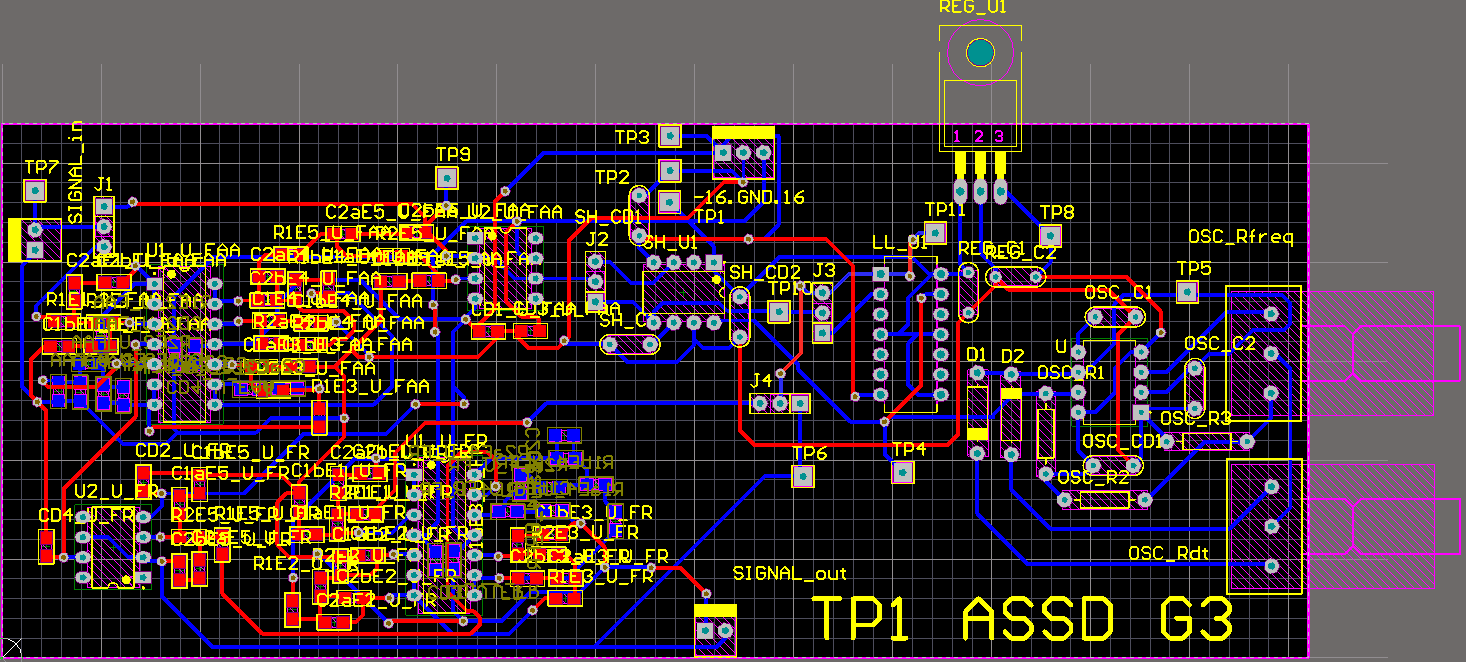
\includegraphics[width=1\linewidth]{ImagenesEjercicio6/placa.png}
	\caption{PCB altium.}
	\label{fig:pcb}
\end{figure}